\documentclass[main.tex]{subfiles} % Subfile-Class

%==============================================================================%
%                                   Subfile                                    %
%==============================================================================%

\begin{document}

% Template

\subsubsection{Steuerungstopologie und Gesamtübersicht}~\label{sec:Gesamtuebersicht_Elektro}

Abbildung~\ref{fig:Gesamtuebersicht_vereinfacht} zeigt das Elektrokonzept in
einem kleinen Detaillierungsgrad. Ziel ist es, im Sinne der Gewaltenteilung
jede Steuerungseinheit für sich abgeschlossen zu betrachten. Die Eingangs
geplante Aufteilung der Hardware in den Greif und den Antriebsprozess wurde im
Laufe von Pren2 zwecks Komponentenvielfaltreduktion zusammengeführt. Daher
lassen sich die Steueraufgaben nun trennen in \textit{Hardwareansteuerung} und
\textit{Intelligenz / Navigation}.

\begin{figure}[H]
    \centering
    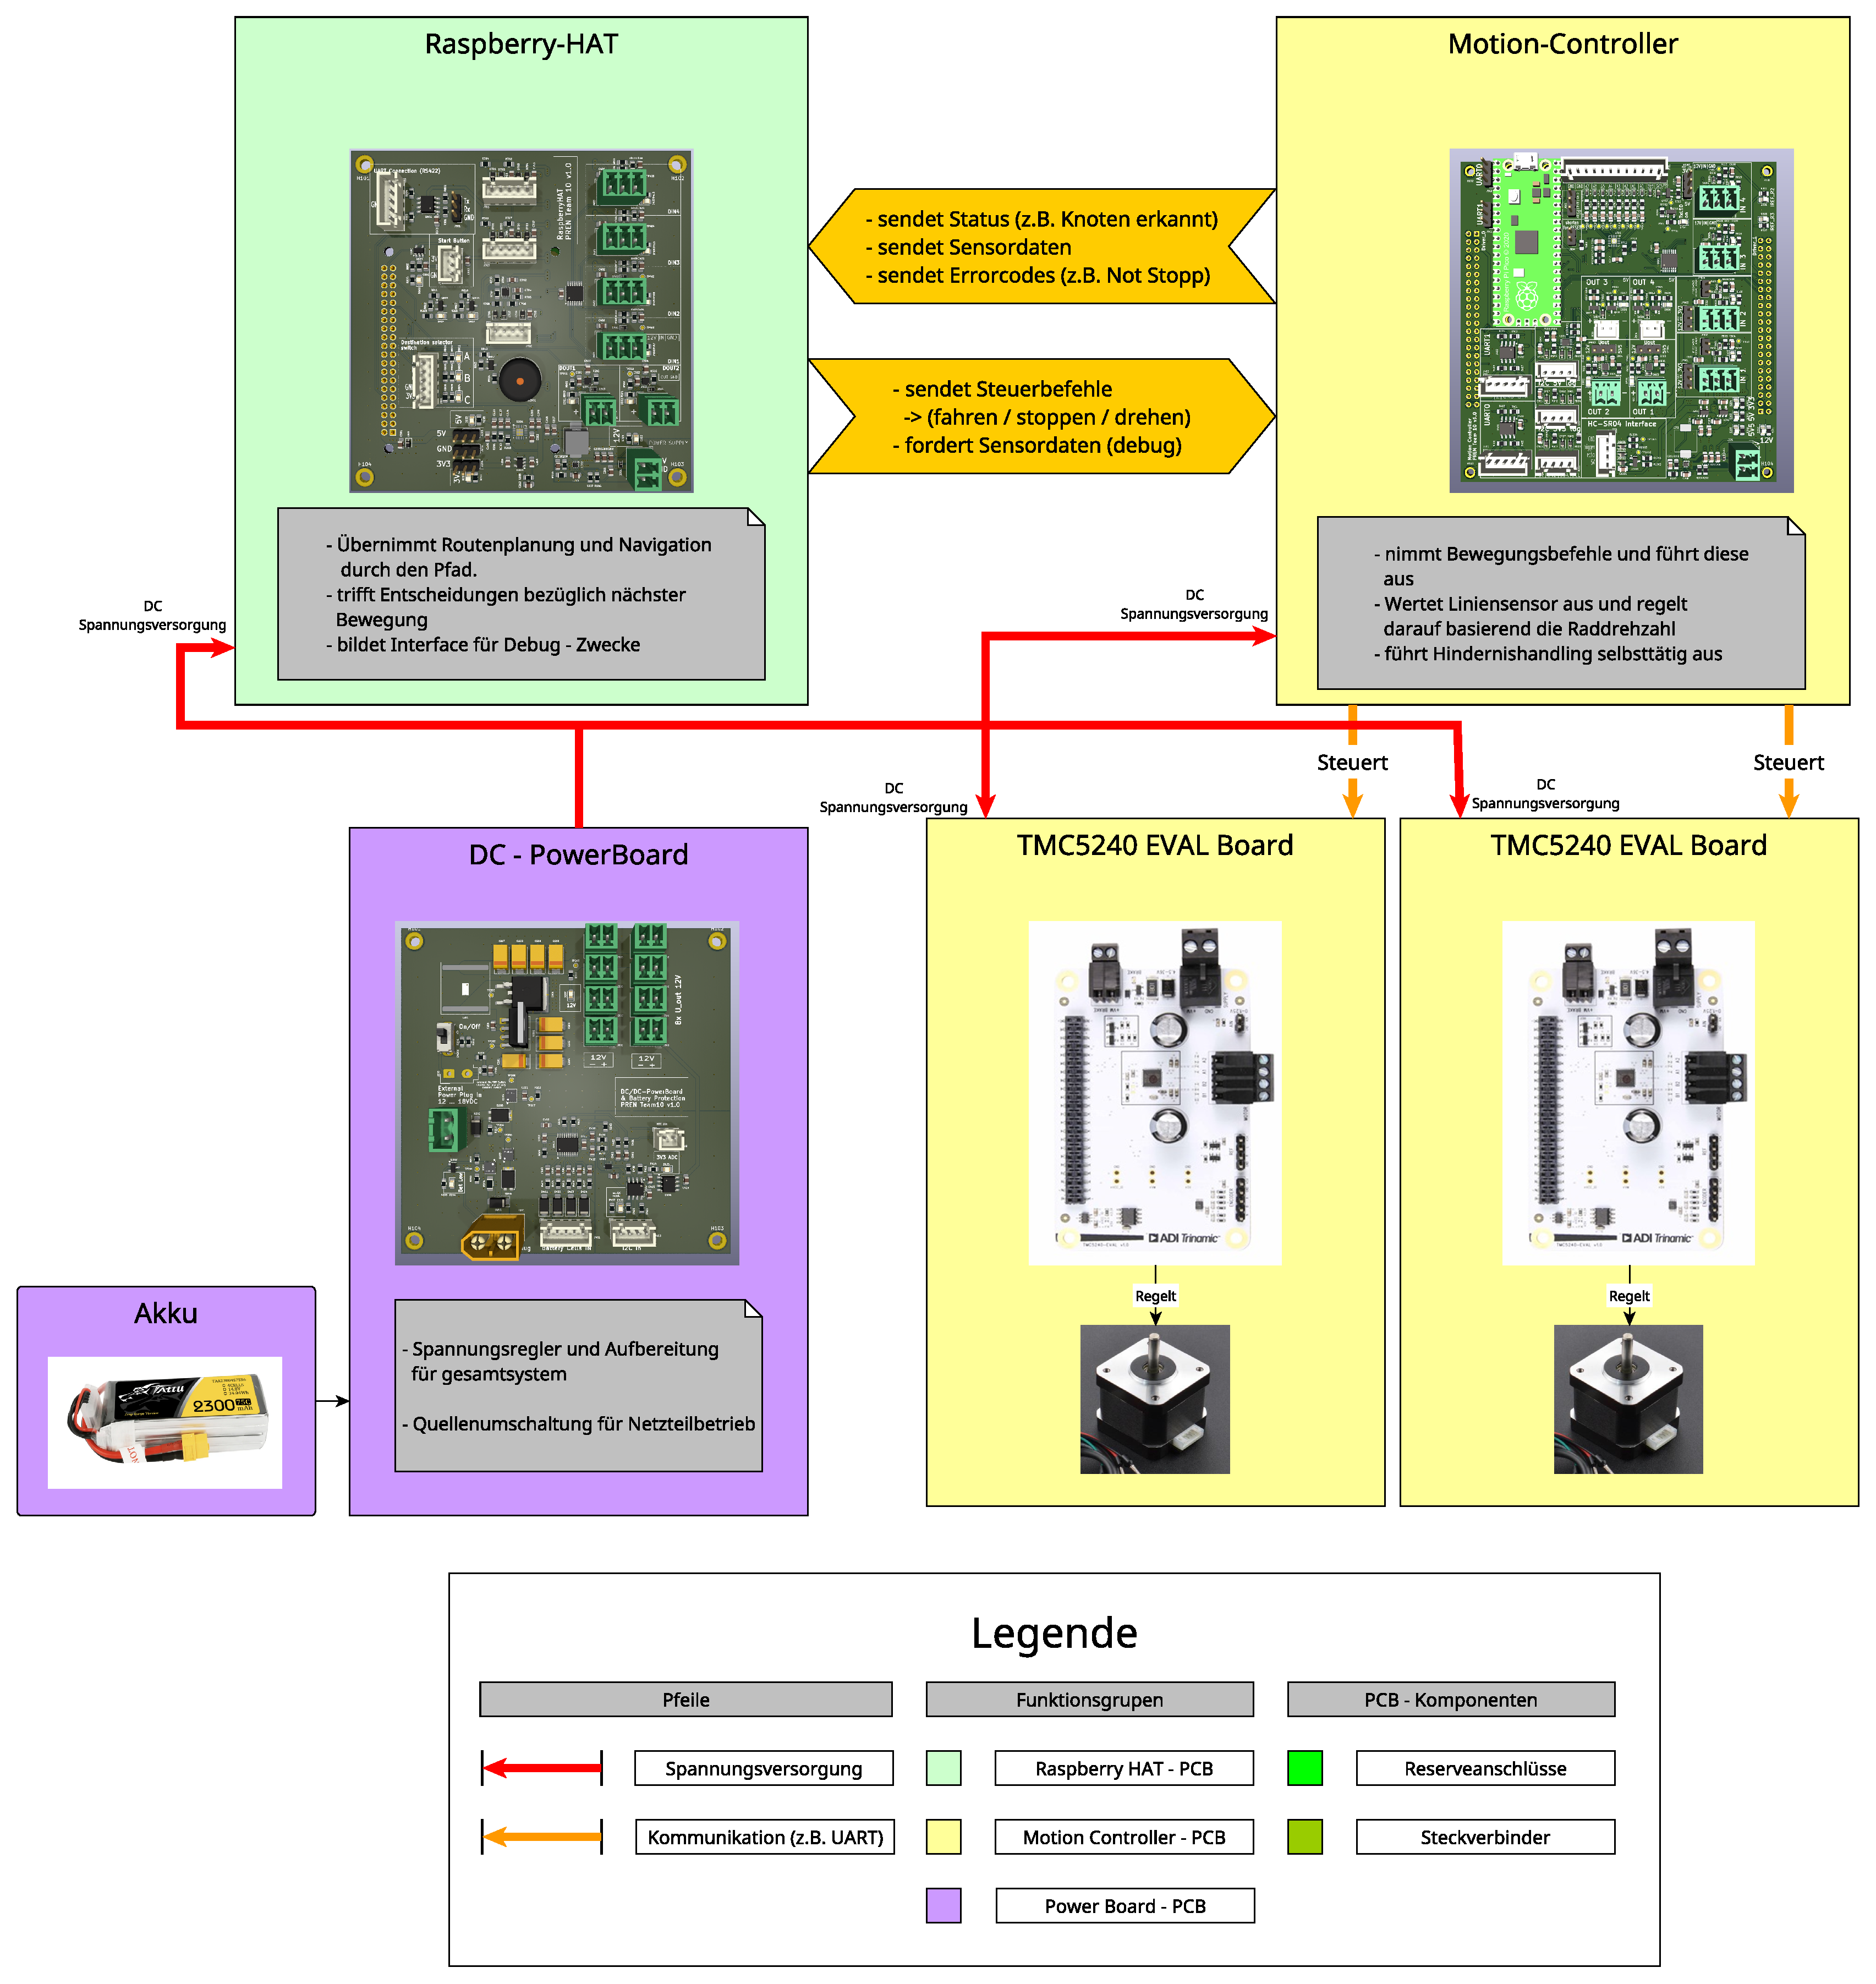
\includegraphics[width = 1\linewidth]{./fig_Elektronik_Gesamtuebersicht/Blockschaltbild_Elektro_vereinfacht.pdf}
    \caption{Vereinfachte Gesamtübersicht Elektronikkonzept}~\label{fig:Gesamtuebersicht_vereinfacht}
\end{figure}

In Anhang~\ref{apdx:Blockschaltbild_Elektrokonzept} ist dieses Blockschaltbild
nochmals mit einem höheren Detaillierungsgrad aufgeführt.

\subsubsection*{Die verschiedenen Funktionsgruppen und ihre PCBs}
Es werden total die 3 folgenden Funktionsgruppen unterschieden:

\begin{description}
    \item[Raspberry HAT] Dieser PCB hat die Aufgabe, die nötige Peripherie für den
        Raspberry Pi zur Verfügung zu stellen. Dies beinhaltet die Anbindung
        verschiedener Taster an die entsprechenden GPIOs sowie eine
        Spannungsversorgung. Der Raspberry Pi soll ausserdem über einen Summer Signale
        wie das Erreichen des Zielpunktes signalisieren können.
    \item[Motion Controller] Der MotionController bietet die Schnittstelle zwischen der
        Hardware des Roboters, wie den Motoren, dem Greifer und den Sensoren und der
        Steuerung im RaspberryHat. Dazu abstrahiert er die Ansteuerung dieser
        Peripherie auf das eigens konzipierte \textit{prain\_uart}-Protokoll.
    \item[Power Board] Das Power Board bietet die Spannungsaufbereitung für den Roboter.
        Hier werden aus den 14.4V Batteriespannung 12V Boardnetzspannung eingeregelt.
        Ausbalanciert wird die Batterie über ein externes Ladegerät. Wird ein 14...18V
        Netzteil an diesem Board angeschlossen, wird die Batterie vom Fahrzeug
        getrennt, was Einricht- und Entwicklungsarbeiten erlaubt, ohne dass dazu eine
        Batterie benötigt wird.
\end{description}

\subsubsection{Prain\_UART - Protokoll}

Zur Kommunikation zwischen den einzelnen Steuerungen ist ein eigenes
Kommunikationsprotokoll entwickelt und implementiert. Als Übertragungskanal
dient der UART-Kanal des Raspberry Pi \& Raspberry Pico. Wie dieses Protokoll
genau funktioniert, ist im Abschnitt~\ref{sec:prain_uart} detailliert
ausgeführt. Es war geplant die Kommunikation über einen RS422 Bus zu
übertragen, eine einfache Single-Ended Übertragung hat sich bei Versuchen
allerdings als vollkommen ausreichend gezeigt.

\subsubsection*{Bordnetz}

Auf dieses wird in der Sektion~\ref{sec:PowerManagement} im Detail eingegangen.
Kurz ausgedrückt besitzt jedes Board eine eigene Spannungswandlung von 12V auf
5V respektive 3.3V, welche vom Power Board zur Verfügung gestellt werden. Damit
steht jedem Board eine grosse Reserve bei der Spannungsversorgung zu verfügung
und ein Anlauf der Motoren kann vom Boardnetz abgefangen werden, ohne dass die
Spannung auf den Boards zusammenbricht.

\subsubsection*{Notstopp}

Die Aufgabenstellung fordert einen Notstopp für das gesamte System, durch
welchen alle gefährlichen Bewegungen des Roboters eingestellt werden. In diesem
Fahrzeug ist dieser in Form von Software umgesetzt. Ein erkanntes
Notstopp-Signal löst einen Broadcast an alle Tasks der Firmware aus, die auf
dem MotionController für Bewegungen zuständig sind. Im Anschluss ist der
MotionController solange blockiert, wie der Notstopp betätigt ist. Dadurch
befindet sich die Antriebselektronik immer in einem definierten Zustand und
alle Steuerungen können ordnungsgemäss heruntergefahren und deinitialisiert
werden.

Die Anordnung des Notstopps ist in Abbildung ersichtlich. % TODO// Abbildung! 

\subsubsection*{Sensoren und Aktoren}

Das Fahrzeug ist mit einem Ultraschallsensor zur Erkennung von Barrieren, einem
LIDAR zur Erkennung von Pylonen über Hindernisse Hinweg, einer Kamera zur
Erkennung von Knotenabgängen während der Annäherung an diese sowie Endschaltern
zur Erfassung der aktuellen Greiferposition ausgestattet.

Die Ansteuerung der Motoren erfolgt über zwei Motorentreiber der Firma
ADI-Trinamic, die vom Motion Controller aus angesteuert werden. Als Motoren
sind 2-Phasen-Hybrid-Schrittmotoren im Einsatz, die über die Treiber im
Open-Loop-Betrieb angesteuert werden. Durch diese Motoren ist eine präzise
Positionierung des Fahrzeugs im Parcours möglich, was besonders beim
Hindernishandling von Vorteil ist.

\end{document}
